\section{Результаты}
Для расчета нормальных колебаний была добавлена опция HSSEND=.TRUE. (в поле \$STATPT\$). По-умолчанию GAMESS рассчитывает гессиан аналитически. Однако рассчитать нормальные колебания c аналитическим гессианом не получилось. Поэтому была добавлена опция METHOD=SEMINUM (в поле \$FORCE\$). С этой опцией градиент считается аналитически, а гессиан -- численно.

Ниже приведены данные о колебательных модах молекулы, взятые из раздела NORMAL COORDINATE ANALYSIS IN THE HARMONIC APPROXIMATION.
\begin{table}[H]
    \caption{Нормальные колебания молекулы}
    \begin{center}
    \label{tab:my-table}
    \resizebox{\textwidth}{!}{%
    \begin{tabular}{|c|c|c|c|c|}
    \hline
    № колебания & Частота, см^{-1} & \begin{tabular}[c]{@{}c@{}}Какой группе\\ атомов соответствует\end{tabular} & Форма колебания & \begin{tabular}[c]{@{}c@{}}Разрешены\\ в ИК-спектрах\end{tabular} \\ \hline
     7  & 161.19 & F1, F2 & Неплоское & +  \\ \hline
     8  & 340.43 & F1, F2 & Плоское & + \\ \hline
     9  & 374.98 & C1-C6, F1, F2 & Неплоское & - \\ \hline
     10 & 440.29 & C1-C6, F1, F2 & Плоское & - \\ \hline
     11 & 447.31 & \begin{tabular}[c]{@{}c@{}}H1, H3, C1, C3, C5\\ H2, H4, C2, C6, C4\end{tabular} & Неплоское & - \\ \hline
     12 & 455.96 & F1, C1, F2, C2 & Плоское & - \\ \hline
     13 & 516.81 & \begin{tabular}[c]{@{}c@{}}H1, H3, C1\\ H2, H4, C2\end{tabular} & Неплоское & + \\ \hline
     14 & 658.98 & C3, C4, C5, C6 & Плоское & - \\ \hline
     15 & 703.29& \begin{tabular}[c]{@{}c@{}}H1, H3, C1, C3, C5\\ H2, H4, C2, C6, C4\end{tabular} & Неплоское & - \\ \hline
     16 & 733.82& \begin{tabular}[c]{@{}c@{}}H1, H3, F1, C3, C5\\ H2, H4, F2, C6, C4\end{tabular} & Плоское & + \\ \hline
     17 & 839.55& H1, H2, H3, H4 & Неплоское & - \\ \hline
     18 & 860.32 & \begin{tabular}[c]{@{}c@{}}H1, H3, С1 \\ H2, H4, С2\end{tabular} & Неплоское & + \\ \hline
     19 & 867.16 & \begin{tabular}[c]{@{}c@{}}H1, H3, C3, C5 \\ H2, H4, С4, C6\end{tabular} & Плоское & - \\ \hline
     20 & 965.54 & H1-H4 & Плоское & - \\ \hline
     21 & 987.51 & H1-H4 & Плоское & - \\ \hline
     22 & 1046.44 & \begin{tabular}[c]{@{}c@{}}H1, H3, C3, C5 \\ H2, H4, С4, C6\end{tabular} & Плоское & + \\ \hline
     23 & 1132.09 & H1-H4 & Плоское & + \\ \hline
     24 & 1193.39 & H1-H4 & Плоское & - \\ \hline
     25 & 1243.31 & Все атомы & Плоское & + \\ \hline
     26 & 1276.32 & Все атомы & Плоское & - \\ \hline
     27 & 1335.91 & H1-H4 & Плоское & - \\ \hline
     28 & 1374.23 & С1-С6 & Плоское & + \\ \hline
     29 & 1458.52 & С1-С6, H1-H4 & Плоское & + \\ \hline
     30 & 1559.91 & С1-С6, H1-H4 & Плоское & + \\ \hline
     31 & 1664.12 & С1-С6, H1-H4 & Плоское & - \\ \hline
     32 & 1668.41 & С1-С6, H1-H4 & Плоское & - \\ \hline
     33 & 3237.44 & H1, H2, H3, H4 & Валентное плоское & + \\ \hline
     34 & 3239.22 & H1, H2, H3, H4 & Валентное плоское & - \\ \hline
     35 & 3251.96 & H1, H2, H3, H4 & Валентное плоское & + \\ \hline
     36 & 3254.06 & H1, H2, H3, H4 & Валентное плоское & - \\ \hline
    \end{tabular}%
    }
    \end{center}{}
\end{table}

\begin{figure}[H]
    \centering
    \captionsetup{justification=centering}
    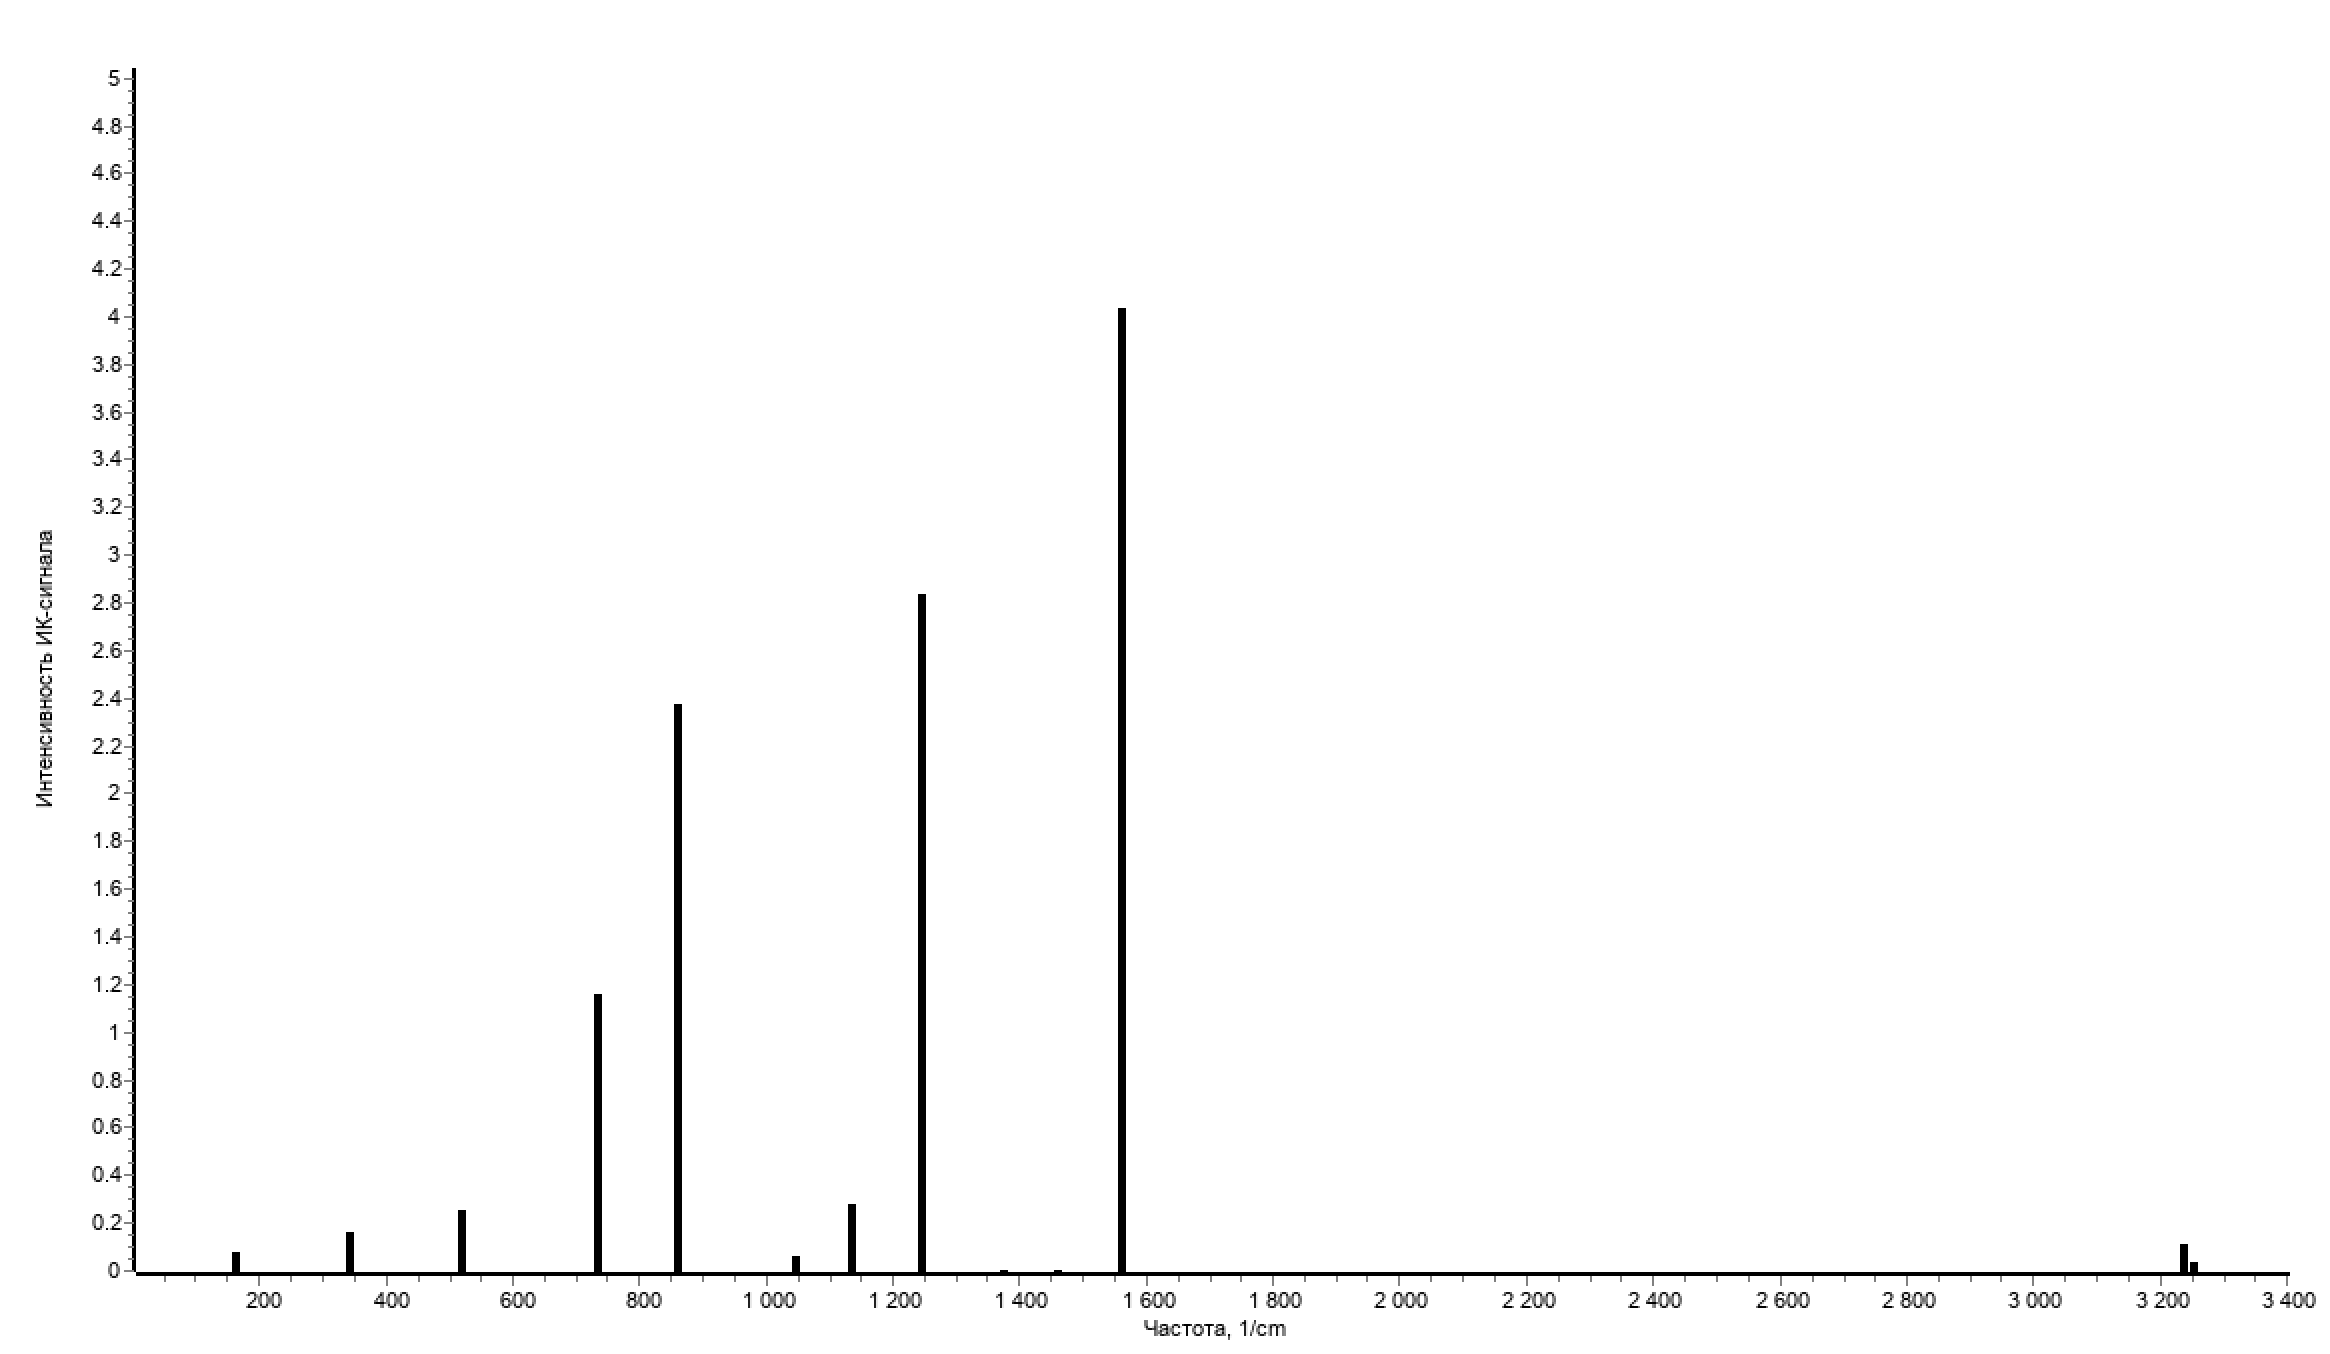
\includegraphics[scale=0.4]{fig/1}
    \caption{ИК-спектр молекулы}
\end{figure}